\documentclass[a4paper,12pt]{report}

\usepackage[utf8]{inputenc}
\usepackage[a4paper,margin=24mm]{geometry}
\usepackage[skip=10pt plus1pt, indent=20pt]{parskip}
\usepackage[colorlinks=true,allcolors=blue,urlcolor=magenta]{hyperref}

\usepackage{caption}
\usepackage{indentfirst,setspace,subcaption}
\usepackage{amsmath,amssymb,graphicx,xcolor,url}
\usepackage{fancyhdr,tocbasic,titlesec,minted,listings}
\usepackage{algorithm}
\usepackage{algpseudocode}

\renewcommand{\thesection}{\arabic{section}}

\renewcommand{\thesection}{\arabic{section}}
\renewcommand{\listoflistingscaption}{Source code}

\newcommand{\codeimport}{\inputminted[breakanywhere=true,breaklines=true]}


% Code highlighting
\usemintedstyle{one-dark}
\setminted{frame=lines,
  framesep=2mm,
  baselinestretch=1.2,
  fontsize=\footnotesize,
  linenos,
  breakanywhere,
  breaklines,
  mathescape
}

% Header and footer styling
\pagestyle{fancy}
\setlength{\headheight}{18pt}
\fancyhf{}
\fancyhead[R]{\nouppercase\rightmark\hfill~Project 01: Ares's Adventure Report}
\fancyfoot[C]{\hfill\thepage\hfill}

% TOC styling
\DeclareTOCStyleEntry[
  indent=12pt,
  level=1
]{largetocline}{section}

% Title page data
\title{Project 01: Ares's Adventure Report}
\author{\begin{tabular}{r c}
  Ngo Nguyen The Khoa & 23127065\\
  Bui Minh Duy       & 23127040\\
  Nguyen Le Ho Anh Khoa      & 23127211\\
\end{tabular}}
\date{March 3, 2025}

\begin{document}
\newenvironment{codewithlisting}[2]{
	\begin{listing}[!ht]
		\caption[#1]{#1}
		\label{listing:#2}}{\end{listing}
}


% Title page and TOC
\thispagestyle{empty}
\begin{titlepage}
	\begin{center}
		\makeatletter
		\newcommand{\HRule}{\rule{\linewidth}{0.4mm}}

		\textsc{\LARGE Vietnam National University,\\Ho Chi Minh City}\\[1.5cm]
		\textsc{\Large University of Science}\\[0.5cm]
		\textsc{\Large Faculty of Information Technology}\\[1.5cm]

		{\HRule}\\[1cm]
		{\huge \bfseries \@title}\\[0.5cm]
		{\HRule}\\[2cm]

		\textsc{\large CS14003 --  Introduction to Artificial Intelligence}\\[0.5cm]

		\vfill\vfill\vfill

		{\large \@author}\\[1.5cm]
		{\large \@date}
		\makeatother
	\end{center}
\end{titlepage}

\tableofcontents\thispagestyle{empty}

% Report contents
\pagebreak
\section{Group Information}
\begin{itemize}
  \item \textbf{Subject:} Introduction to Artificial Intelligence.
  \item \textbf{Class:} 23CLC09.
  \item \textbf{Lecturer:} Bui Duy Dang, Le Nhut Nam.
  \item \textbf{Team members:}
        \begin{center}
          \renewcommand{\arraystretch}{1.5}
          \begin{tabular}{|c|l|c|l|}
            \hline
            \textbf{No.} & \textbf{Fullname}     & \textbf{Student ID} & \textbf{Email}                                                         \\\hline
            1            & Ngo Nguyen The Khoa   & 23127065            & \href{mailto:nntkhoa23@clc.fitus.edu.vn}{nntkhoa23@clc.fitus.edu.vn}   \\\hline
            2            & Bui Minh Duy          & 23127040            & \href{mailto:bmduy23@clc.fitus.edu.vn}{bmduy23@clc.fitus.edu.vn}       \\\hline
            3            & Nguyen Le Ho Anh Khoa & 23127211            & \href{mailto:nlhakhoa23@clc.fitus.edu.vn}{nlhakhoa23@clc.fitus.edu.vn} \\\hline
          \end{tabular}
        \end{center}
\end{itemize}

\section{Project Information}
\begin{itemize}
  \item \textbf{Name:} Ares.
  \item \textbf{Developing Environment:} Visual Studio Code (Windows).
  \item \textbf{Programming Language:} Python.
  \item \textbf{Libraries and Tools:}
        \begin{itemize}
          \item \href{https://rye.astral.sh/}{\textbf{rye:}} A comprehensive project and package management solution for Python.
          \item \href{https://customtkinter.tomschimansky.com/}{\textbf{CustomTkinter:}} GUI library.
        \end{itemize}
\end{itemize}


\pagebreak
\section{Work assignment table}
\begin{center}
  \renewcommand{\arraystretch}{1.5}
  \begin{tabular}{|c|p{\dimexpr0.55\linewidth-2\tabcolsep}|r|c|}
    \hline
    \textbf{No.} & \textbf{Task Description}                                         & \textbf{Assigned to} & \textbf{Rate} \\\hline
    1            & Implement BFS, DFS                                                & Minh Duy             & 100\%         \\\hline
    2            & Implement UCS, Dijkstra                                           & Anh Khoa             & 100\%         \\\hline
    3            & Implement A*, GBFS                                                & The Khoa             & 100\%         \\\hline
    4            & Implement Swarm                                                   & Anh Khoa             & 100\%         \\\hline
    5            & Optimize heuristic function using Hungarian for min-matching      & The Khoa, Minh Duy   & 100\%         \\\hline
    6            & Optimize the number of expanded nodes by using deadlock detection & The Khoa, Anh Khoa   & 100\%         \\\hline
    7            & Video Editing                                                     & Minh Duy             & 100\%         \\\hline
    8            & Report                                                            & All members          & 100\%         \\\hline
  \end{tabular}
\end{center}

\pagebreak
\section{Self-evaluation}
\begin{center}
  \renewcommand{\arraystretch}{1.5}
  \begin{tabular}{|l|p{\dimexpr0.8\linewidth-2\tabcolsep}|c|}
    \hline
    \textbf{No.} & \textbf{Criteria}                                                                                                                  & \textbf{Score} \\ \hline
    1            & Implement BFS correctly.                                                                                                           & 100\%          \\ \hline
    2            & Implement DFS correctly.                                                                                                           & 100\%          \\ \hline
    3            & Implement UCS correctly.                                                                                                           & 100\%          \\ \hline
    4            & Implement A* correctly.                                                                                                            & 100\%          \\ \hline
    5            & Implement GBFS correctly.                                                                                                          & 100\%          \\ \hline
    6            & Generate at least 10 test cases for each level with diffenrent attributes.                                                         & 100\%          \\ \hline
    7            & Result (output file and GUI).                                                                                                      & 100\%          \\ \hline
    8            & Video to demonstrate all algorithms for some test cases.                                                                           & 100\%          \\ \hline
    9            & Report.                                                                                                                            & 100\%          \\ \hline
    10           & Implement, written report for Dijkstra's Algorithm, Swarm Algorithm, Convergent Swarm Algorithm and Bidirectional Swarm Algorithm. & 100\%          \\ \hline
  \end{tabular}
\end{center}

\pagebreak
\section{Algorithms' Implementations}
\subsection{BFS Algorithms}
\subsubsection{Introduction}
Breadth-First Search (BFS) is a fundamental graph traversal algorithm used to explore nodes in a graph or tree data structure. It operates by visiting all nodes at the current depth level (``breadth'') before moving to nodes at the next depth level. BFS guarantees the shortest path in an unweighted graph, making it highly useful in applications like network routing, social network analysis, and puzzle solving.

\subsubsection{Algorithm Overview}
\begin{enumerate}
	\item Key Principles
	      \begin{description}
		      \item \textbf{Queue Data Structure:} BFS uses a queue (First-In-First-Out principle) to track nodes to be explored.
		      \item \textbf{Layer-by-Layer Exploration:} Nodes are visited level by level, starting from the root (or source node).
		      \item \textbf{Visited Tracking:} A visited array or hash map prevents reprocessing nodes, avoiding cycles.
	      \end{description}

	\item Steps of BFS
	      \begin{enumerate}
		      \item \textbf{Initialize:}
		            \begin{description}
			            \item Select a starting node (root).
			            \item Create a queue and add the root node.
			            \item Mark the root as visited.
		            \end{description}
		      \item \textbf{Loop Until Queue is Empty:}
		            \begin{description}
			            \item Dequeue the front node.
			            \item Process the node (e.g., print its value).
			            \item Enqueue all adjacent unvisited nodes and mark them as visited.
		            \end{description}
		      \item \textbf{Terminate:} When the queue is empty, traversal is complete.
	      \end{enumerate}
\end{enumerate}

\subsubsection{Pseudocode}
\begin{lstlisting}
	BFS(Graph G, StartNode):
		Initialize empty Queue Q
		Initialize empty Set visited
		Q.enqueue(StartNode)
		visited.add(StartNode)
	
		while Q is not empty:
			current = Q.dequeue()
			Process(current)  // e.g., print node
	
			for each neighbor in G.adjacentNodes(current):
				if neighbor not in visited:
					visited.add(neighbor)
					Q.enqueue(neighbor)
	\end{lstlisting}

\subsubsection{Time and Space Complexity}
\textbf{Time Complexity:} $O(V + E)$, where $V$ is the number of vertices and $E$ is the number of edges. Each node and edge is processed once.

\textbf{Space Complexity:} $O(V)$ in the worst case, as the queue stores all nodes at the widest level of the graph.

\subsubsection{Applications}
\begin{itemize}
	\item \textbf{Shortest Path in Unweighted Graphs:} BFS guarantees the minimum number of edges between two nodes.
	\item \textbf{Social Networks:} Find connections or degrees of separation between users.
	\item \textbf{Web Crawling:} Index web pages level by level.
	\item \textbf{Cycle Detection:} Identify cycles in undirected graphs.
	\item \textbf{Puzzle Solving:} Solve problems like the water jug'' or maze pathfinding'' efficiently.
\end{itemize}

\subsubsection{Advantages and Limitations}
\begin{itemize}

	\item \textbf{Advantages}
	      \begin{itemize}
		      \item Optimal for finding the shortest path in unweighted graphs.
		      \item Systematic and complete (guarantees finding a solution if one exists).
	      \end{itemize}

	\item \textbf{Limitations}
	      \begin{itemize}
		      \item High memory consumption for wide graphs due to queue storage.
		      \item Inefficient for deep graphs compared to Depth-First Search (DFS).
	      \end{itemize}

\end{itemize}
\subsubsection{Comparison with Depth-First Search (DFS)}
\begin{center}
	\begin{tabular}{|c|c|c|}
		\hline
		\textbf{Criteria} & \textbf{BFS}                    & \textbf{DFS}                      \\
		\hline
		Data Structure    & Queue                           & Stack                             \\
		\hline
		Optimal Path      & Yes (unweighted graphs)         & No                                \\
		\hline
		Memory Usage      & Higher (stores all neighbors)   & Lower (depth-based)               \\
		\hline
		Use Cases         & Shortest path, network analysis & Topological sorting, backtracking \\
		\hline
	\end{tabular}
\end{center}

\subsubsection{Conclusion}
BFS is a versatile algorithm with wide-ranging applications in computer science and real-world systems. Its ability to systematically explore graphs layer by layer makes it indispensable for problems requiring shortest-path solutions or comprehensive traversal. However, its memory constraints necessitate careful consideration when applied to large-scale datasets.


\subsection{Depth First Search}
\noindent Depth First Search (DFS) is a special case of backtracking search algorithm. The search starts from the root and proceeds to the farthest node before backtracking. The difference between this and the backtracking is that this stops the search once a goal is reached and does not care if it is not minimum.

\begin{figure}[H]
	\centering
	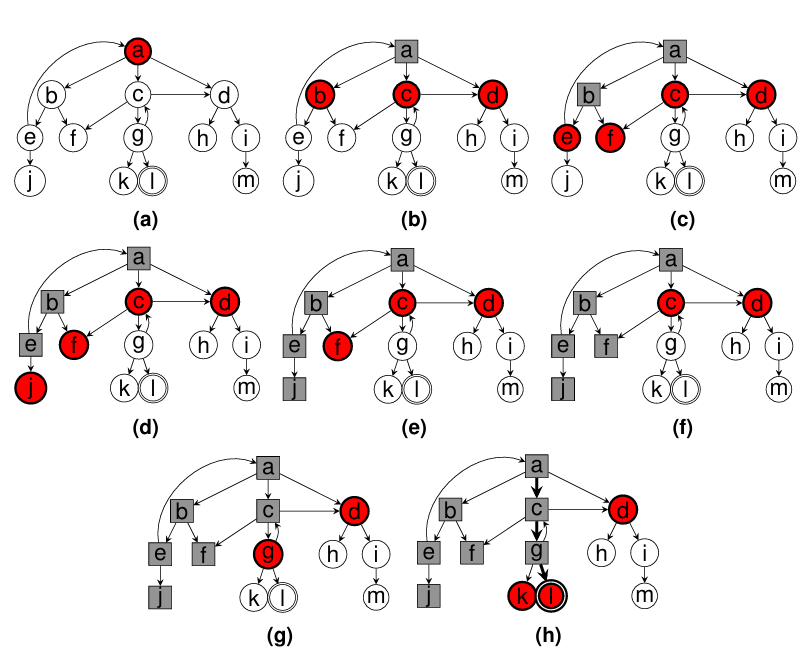
\includegraphics[width=0.8\textwidth]{./imgs/dfs.png}
	\caption{Depth First Search}
\end{figure}

\subsubsection{Pseudocode}
\begin{algorithm}[H]
	\caption{Depth First Search (\textit{start, goal})}
	\label{alg:dfs}
	\begin{algorithmic}[1]
	\State stack $\gets$ [start]
	\While {stack is not empty}
		\State node $\gets$ pop(stack)
		\If {node = goal}
			\State return path
		\EndIf
		\ForAll {neighbor in valid moves}
			\If {neighbor not visited}
				\State mark neighbor as visited
				\State push(stack, neighbor)
			\EndIf
		\EndFor
	\EndWhile
	\State return failure
	\end{algorithmic}
\end{algorithm}

\subsubsection{Implementation}

\subsubsection{Time and Space Complexity}
\subsection{Uniform Cost Search}
\begin{flushleft}
	Uniform Cost Search (UCS) is a graph traversal algorithm that expands the least-cost node first.

	Unlike BFS and DFS, UCS considers edge weights, ensuring that the path found is the shortest in terms of total cost. It is functionally equivalent to Dijkstra's algorithm when used for single-source shortest path problems.

	UCS operates using a priority queue, where nodes are processed based on their cumulative path cost, making it ideal for finding optimal solutions in weighted graphs.
\end{flushleft}

\subsubsection{Pseudocode}
\begin{algorithm}[H]
	\caption{Uniform Cost Search (\textit{start, goal})}
	\label{alg:ucs}
	\begin{algorithmic}[1]
		\State priority queue \(\gets\) [(start, cost = 0)]
		\While {priority queue is not empty}
		\State (node, cost) \(\gets\) dequeue(priority queue)
		\If {node = goal}
		\State return path
		\EndIf
		\ForAll {neighbor in valid moves}
		\State new cost \(\gets\) cost + move cost
		\If {neighbor not visited or new cost \(<\) previous cost}
		\State mark neighbor as visited
		\State enqueue(priority queue, (neighbor, new cost))
		\EndIf
		\EndFor
		\EndWhile
		\State return failure
	\end{algorithmic}
\end{algorithm}

\subsubsection{Implementation}
\begin{itemize}
	\item \textbf{\_\_init\_\_(\ldots)}
	      Initializes the Uniform Cost Search (UCS) algorithm with grid dimensions, matrix representation, initial player position, stone positions, and switch positions. It also includes an option for deadlock detection. The initial state's cost \( g \) is set to zero.

	\item \textbf{search()}
	      Implements the UCS algorithm using a priority queue (min-heap). The function expands the node with the lowest accumulated cost \( g \) at each step. It explores all possible states, updating costs and storing them in a hash table for efficient lookup.

	\item \textbf{handle(new\_state, closed, frontier, state\_hash\_table)}
	      Manages newly generated states, adding them to the frontier if they have not been visited or updating their cost if a lower-cost path is found.

	\item \textbf{can\_go(current\_state, dir)}
	      Checks whether the player can move in a given direction from the current state without encountering obstacles and deadlock cells.

	\item \textbf{go(current\_state, dir)}
	      Generates a new state by moving the player in the specified direction, updating positions, and recalculating cost values.

	\item \textbf{construct\_path(final\_state)}
	      Reconstructs the sequence of moves leading to the goal state by backtracking from the final state.
\end{itemize}

\subsubsection{Time and Space Complexity}
\textbf{Time Complexity:} \( O(b^C) \), where \( C \) is the cost of the optimal solution. In the worst case, UCS expands all nodes up to the goal depth.

\textbf{Space Complexity:} \( O(b^C) \), as it stores all expanded nodes in memory.

\subsection{Dijkstra's Algorithm}
\begin{flushleft}
	Dijkstra's algorithm is a classic shortest path algorithm that guarantees finding the minimum-cost path from a starting node to all other nodes in a weighted graph.

	It operates by iteratively selecting the node with the lowest cumulative cost and updating the distances of its neighbors.

	Like UCS, Dijkstra's algorithm uses a priority queue, but it is typically employed in broader applications such as routing and network optimization.
\end{flushleft}

\subsubsection{Pseudocode}
\begin{algorithm}[H]
	\caption{Dijkstra's Algorithm (\textit{start, goal})}
	\label{alg:dijkstra}
	\begin{algorithmic}[1]
		\State priority queue \(\gets\) [(start, cost = 0)]
		\State distances[start] \(\gets\) 0
		\While {priority queue is not empty}
		\State (node, cost) \(\gets\) dequeue(priority queue)
		\If {node = goal}
		\State return distances
		\EndIf
		\ForAll {neighbor in valid moves}
		\State new cost \(\gets\) cost + move cost
		\If {new cost \(<\) distances[neighbor]}
		\State distances[neighbor] \(\gets\) new cost
		\State enqueue(priority queue, (neighbor, new cost))
		\EndIf
		\EndFor
		\EndWhile
		\State return distances
	\end{algorithmic}
\end{algorithm}

\subsubsection{Implementation}
\begin{itemize}
	\item \textbf{\_\_init\_\_(\ldots)}
	      Initializes the Dijkstra search algorithm with grid dimensions, matrix representation, initial player position, stone positions, and switch positions. It also includes an option for deadlock detection. The initial state's cost \( g \) is set to zero.

	\item \textbf{search()}
	      Implements Dijkstra's algorithm using a priority queue (min-heap). The function explores states based on the lowest accumulated cost \( g \). It expands nodes by generating successors, updating costs, and maintaining a hash table for efficient state lookup.

	\item \textbf{handle(new\_state, closed, frontier, state\_hash\_table)}
	      Manages newly generated states, checking if they should be added to the frontier or updated in the hash table based on their cost values.

	\item \textbf{can\_go(current\_state, dir)}
	      Checks whether the player can move in a given direction from the current state without encountering obstacles and deadlock cells.

	\item \textbf{go(current\_state, dir)}
	      Generates a new state by moving the player in the specified direction, updating positions, and recalculating cost values.

	\item \textbf{construct\_path(final\_state)}
	      Reconstructs the sequence of moves leading to the goal state by backtracking from the final state.
\end{itemize}

\subsubsection{Time and Space Complexity}
\textbf{Time Complexity:} \( O((V + E) \log V) \), where \( V \) is the number of vertices and \( E \) is the number of edges. Using a priority queue (min-heap) allows efficient updates.

\textbf{Space Complexity:} \( O(V + E) \), as it stores all nodes and edges in the graph.

\subsection{A* Search with heuristic}
\noindent The A* algorithm is a widely used technique for pathfinding and graph traversal. It relies heavily on heuristics to estimate the future cost of reaching the goal. Essentially, A* extends uniform cost search by incorporating a heuristic function to guide its path selection, making it more efficient in many cases. The choice of heuristic depends on the specific problem domain, highlighting the importance of domain knowledge. For A* to be consistent, the modified cost function must always remain greater than zero.

\begin{figure}[H]
	\centering
	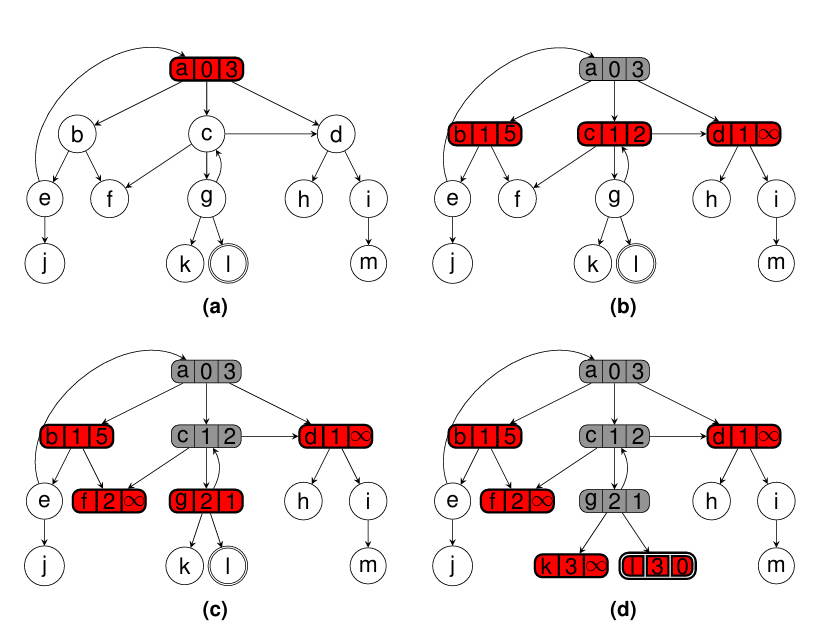
\includegraphics[width=0.8\textwidth]{./imgs/astar.png}
	\caption{A* Algorithm}
\end{figure}

\subsubsection{Pseudocode}
\begin{algorithm}[H]
	\caption{A* Search (\textit{start, goal, heuristic})}
	\label{alg:astar}
	\begin{algorithmic}[1]
		\State priority queue \(\gets\) [(start, cost = 0, estimated total cost = heuristic(start))]
		\While {priority queue is not empty}
		\State (node, cost) \(\gets\) dequeue(priority queue)
		\If {node = goal}
		\State return path
		\EndIf
		\ForAll {neighbor in valid moves}
		\State new cost \(\gets\) cost + move cost
		\State estimated total cost \(\gets\) new cost + heuristic(neighbor)
		\If {neighbor not visited or new cost \(<\) previous cost}
		\State mark neighbor as visited
		\State enqueue(priority queue, (neighbor, new cost, estimated total cost))
		\EndIf
		\EndFor
		\EndWhile
		\State return failure
	\end{algorithmic}
\end{algorithm}

\subsubsection{Implementation}
\begin{itemize}
	\item \textbf{\_\_init\_\_(\ldots)}
	      Initializes the A* search algorithm with grid dimensions, matrix representation, initial player position, stone positions, and switch positions. It also includes options for deadlock detection and heuristic optimization.

	\item \textbf{search()}
	      Implements the A* search algorithm using a priority queue (min-heap). The function explores states by selecting the one with the lowest cost \(f = g + h\). It expands nodes by generating successors, updating costs, and maintaining a hash table for efficient state lookup.

	\item \textbf{handle(new\_state, closed, frontier, state\_hash\_table)}
	      Manages newly generated states, checking if they should be added to the frontier or updated in the hash table based on their cost values.

	\item \textbf{heuristic(stones\_pos, switches\_pos)}
	      Computes the heuristic function to estimate the cost to reach the goal. It selects between the Hungarian heuristic and Manhattan heuristic based on the optimization flag.

	\item \textbf{mahattan\_heuristic(stones\_pos, switches\_pos)}
	      Calculates the heuristic using the Manhattan distance, summing up the minimum distances from each stone to a switch.

	\item \textbf{hungarian\_heuristic(stones\_pos, switches\_pos)}
	      Uses the Hungarian algorithm to optimally assign stones to switches, minimizing the total weighted Manhattan distance.

	\item \textbf{can\_go(current\_state, dir)}
	      Checks whether the player can move in a given direction from the current state without encountering obstacles and deadlock cells.

	\item \textbf{go(current\_state, dir, heuristic)}
	      Generates a new state by moving the player in the specified direction, updating positions and recalculating heuristic values.

	\item \textbf{construct\_path(final\_state)}
	      Reconstructs the sequence of moves leading to the goal state by backtracking from the final state.

\end{itemize}

\subsubsection{Time and Space Complexity}
\textbf{Time Complexity:} \( O(b^d) \) in the worst case, but with a good heuristic, it can be significantly reduced. If the heuristic is admissible and consistent, A* is optimal and complete.

\textbf{Space Complexity:} \( O(b^d) \), as it keeps all generated nodes in memory.

\subsection{Greedy Best-First Search}
\noindent Greedy Best-First Search is similar to A* algorithm. The difference is that the vertices in the priority queue are ordered only by the estimated remaining distance to the solution. It has to be noted that complete best first search is not optimal.

\begin{figure}
	\centering
	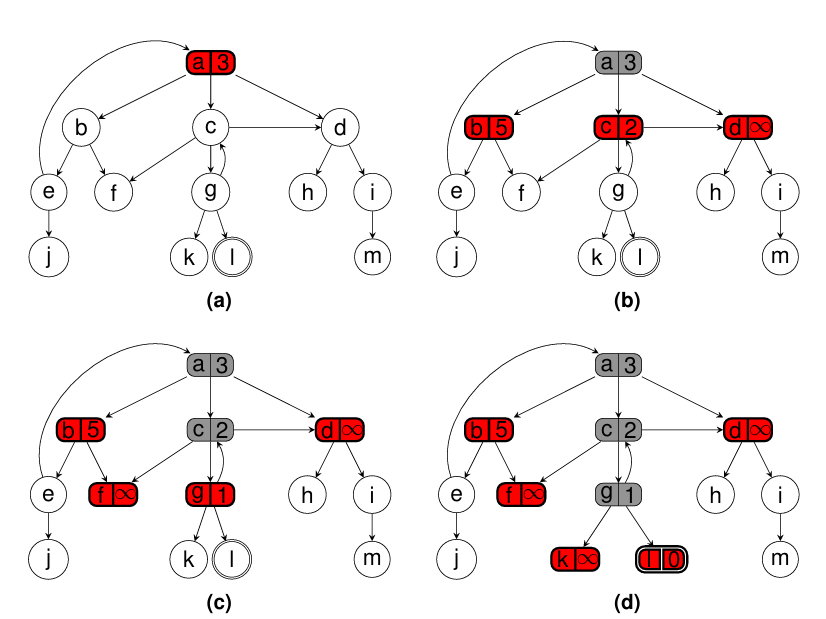
\includegraphics[width=0.8\textwidth]{./imgs/gbfs.png}
	\caption{Greedy Best-First Search}
	\label{fig:GBFS}
\end{figure}

\subsubsection{Pseudocode}
\begin{algorithm}[H]
	\caption{Greedy Best-First Search (\textit{start, goal, heuristic})}
	\label{alg:gbfs}
	\begin{algorithmic}[1]
	\State priority queue $\gets$ [(start, heuristic(start))]
	\While {priority queue is not empty}
		\State node $\gets$ dequeue(priority queue)
		\If {node = goal}
			\State return path
		\EndIf
		\ForAll {neighbor in valid moves}
			\If {neighbor not visited}
				\State mark neighbor as visited
				\State enqueue(priority queue, (neighbor, heuristic(neighbor)))
			\EndIf
		\EndFor
	\EndWhile
	\State return failure
	\end{algorithmic}
\end{algorithm}

\subsubsection{Time and Space Complexity}

\subsection{Swarm Algorithm}

\subsubsection{Pseudocode}

\subsubsection{Implementation}
\begin{itemize}
    \item \textbf{\_\_init\_\_(...)}  
    Initializes the Swarm search algorithm with grid dimensions, matrix representation, initial player position, stone positions, and switch positions. It also includes options for deadlock detection and heuristic optimization.

    \item \textbf{search()}  
    Defines the base search function for Swarm, Swarm Convergent, and Swarm Bidirectional approaches. Currently, the function tracks expanded nodes but does not implement a complete pathfinding process.

    \item \textbf{heuristic(stones\_pos, switches\_pos)}  
    Computes the heuristic function to estimate the cost to reach the goal. The function dynamically selects between the Hungarian heuristic and Manhattan heuristic based on the optimization flag.

    \item \textbf{mahattan\_heuristic(stones\_pos, switches\_pos)}  
    Uses the Manhattan distance to estimate the cost, summing the minimum weighted distances from each stone to a switch.

    \item \textbf{hungarian\_heuristic(stones\_pos, switches\_pos)}  
    Utilizes the Hungarian algorithm to optimally assign stones to switches, minimizing the total weighted Manhattan distance.

    \item \textbf{SwarmConvergent.search()}  
    Implements a variant of Swarm where multiple paths converge towards a solution. Currently, it maintains a set of explored states without a full implementation.

    \item \textbf{SwarmBidirectional.search()}  
    Implements a bidirectional search variant of Swarm, exploring the state space from both the start and goal positions simultaneously. It maintains a set of explored states but lacks a fully developed pathfinding process.

    \item \textbf{AntColonyOptimization.\_\_init\_\_(...)}  
    Initializes the Ant Colony Optimization (ACO) search algorithm with the same parameters as Swarm, allowing for heuristic-based optimizations.

    \item \textbf{AntColonyOptimization.search()}  
    Implements the base ACO search function, tracking expanded states but lacking full functionality.
\end{itemize}

\subsubsection{Time and Space Complexity}
\textbf{Time Complexity:} Highly dependent on the heuristic used. The Hungarian heuristic runs in \( O(n^3) \), while Manhattan distance runs in \( O(n) \). Overall, complexity varies between \( O(n^3) \) and \( O(b^d) \).

\textbf{Space Complexity:} \( O(b^d) \), as it stores visited states.
\subsection{Comparison of Pathfinding Algorithms}

\begin{table}[h]
    \centering
    \begin{tabular}{|c|c|c|c|c|c|}
        \hline
        \textbf{Algorithm} & \textbf{Steps} & \textbf{Weight} & \textbf{Nodes Explored} & \textbf{Time (ms)} & \textbf{Memory} \\
        \hline
        BFS & \textbf{16} & 695 & 5327 & 480.75 & 3.01 MB \\
        \hline
        DFS & 85 & 707 & 444 & 57.66 & 222.34 KB \\
        \hline
        UCS & 24 & \textbf{405} & 20404 & 1560.00 & 13.04 MB \\
        \hline
        A* & 24 & \textbf{405} & 2146 & 382.55 & 1.92 MB \\
        \hline
        GBFS & 26 & \textbf{405} & \textbf{99} & \textbf{16.15} & \textbf{82.50 KB} \\
        \hline
        Dijkstra & 24 & \textbf{405} & 29450 & 2040.00 & 18.28 MB \\
        \hline
    \end{tabular}
    \label{tab:sokoban_comparison}
\end{table}

\begin{figure}[H]
    \centering
    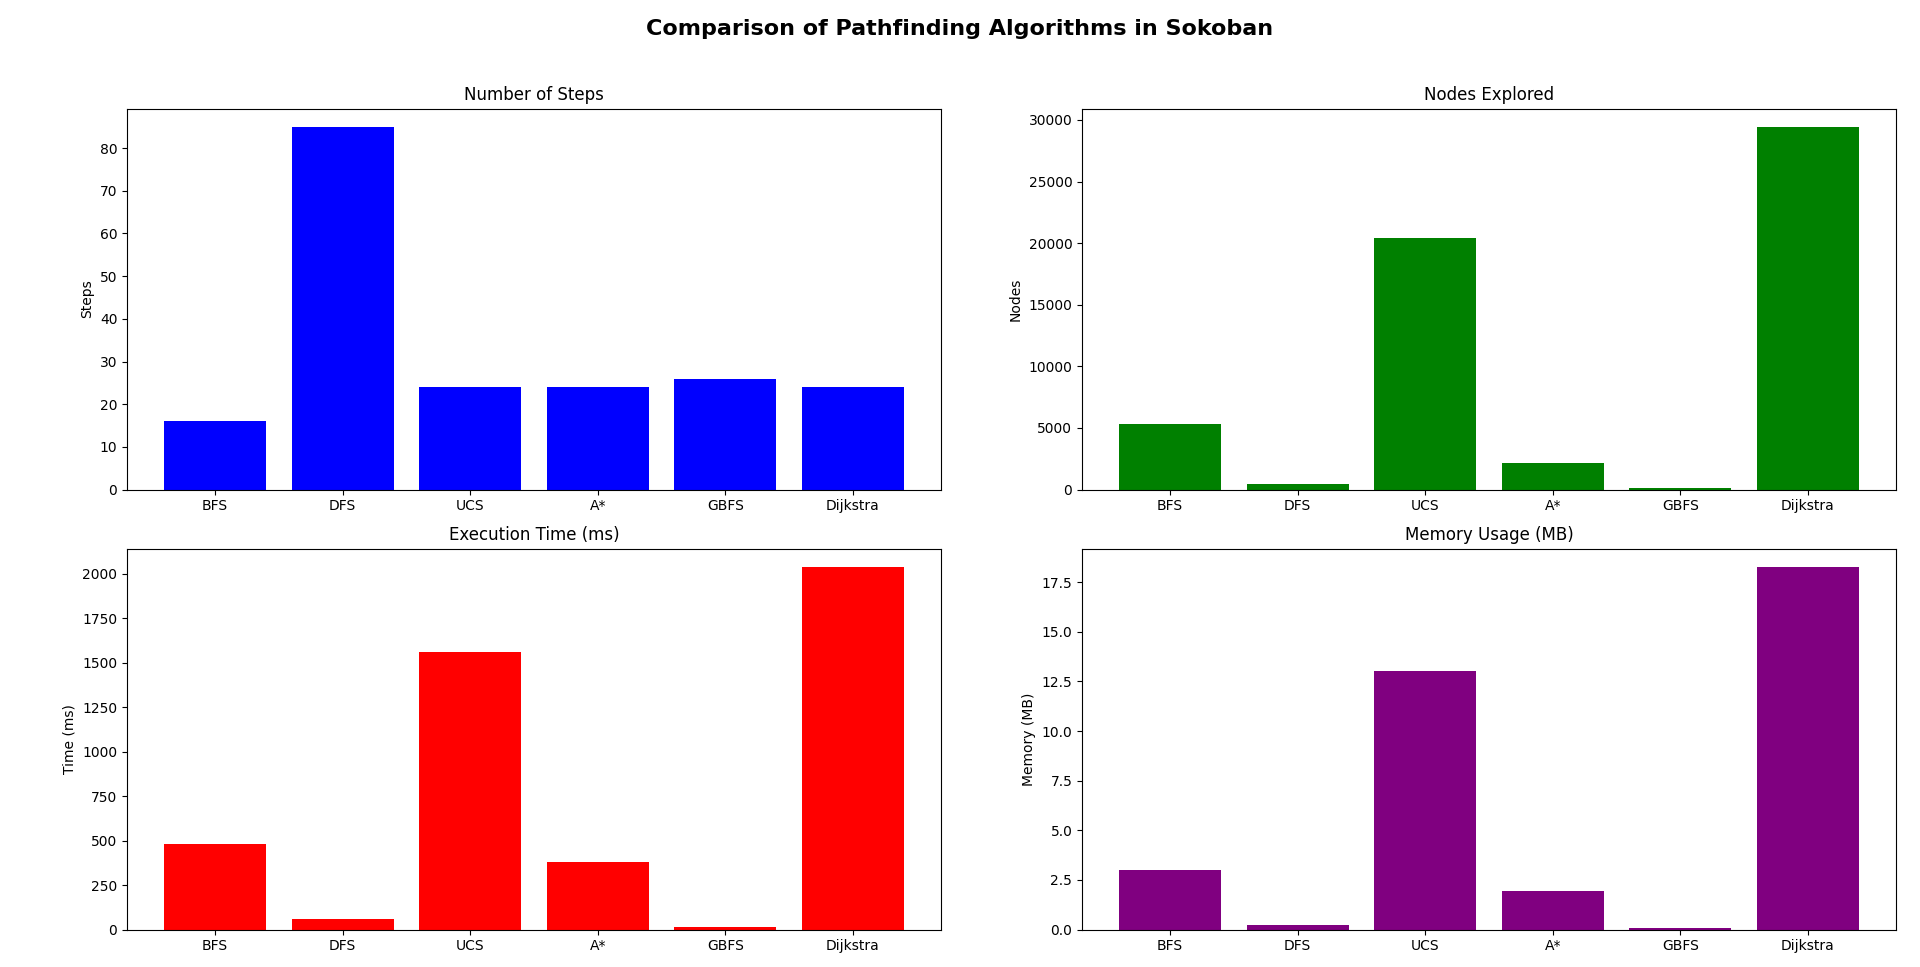
\includegraphics[width=\textwidth]{imgs/bar_graph.png}
    \label{fig:sokoban_comparison}
    \caption{Comparison of Pathfinding Algorithms in Sokoban}
\end{figure}

\subsubsection{Conclusion}
\noindent This report analyzed various search algorithms applied to the Sokoban problem, comparing their efficiency in terms of steps taken, nodes expanded, time, and memory usage. The results indicate that:
\begin{itemize}
    \item \textbf{A*} and \textbf{UCS} produced optimal solutions but required significant memory and processing time.
    \item \textbf{BFS} efficiently found the shortest path in unweighted space but struggled in large graphs.
    \item \textbf{DFS} explored deeply but was inefficient for finding optimal paths.
    \item \textbf{GBFS} was the fastest algorithm but sometimes produced suboptimal solutions due to its greedy nature.
    \item \textbf{Dijkstra’s} algorithm performed similarly to UCS but expanded more nodes due to its exhaustive nature.
    \item \textbf{Swarm-based approaches} showed potential in parallelized exploration, though their performance depends heavily on heuristic design.
\end{itemize}
Future improvements could involve enhanced heuristics, hybrid approaches, or reinforcement learning techniques to further optimize search performance in Sokoban and similar problems.

\pagebreak
\section{App Screenshots}
% \begin{figure}[!ht]
%   \centering
%   \begin{subfigure}{0.46\textwidth}
%     \centering
%     \includegraphics[width=0.9\textwidth]{}
%     \caption{UI 1}
%   \end{subfigure}
%   \hfill
%   \begin{subfigure}{0.46\textwidth}
%     \centering
%     \includegraphics[width=0.9\textwidth]{}
%     \caption{UI 2}
%   \end{subfigure}
%   \caption{UI Caption}
% \end{figure}


% References
\pagebreak
\section{References}
\begin{enumerate}
  \item \href{https://rye.astral.sh/guide/}{Rye documentation}
  \item \href{https://www.pygame.org/docs/}{pygame documentation}
  \item \href{https://github.com/giahuy102/Sokoban-AI-Game/tree/master}{Sokoban AI Game repo}: heavy-inspired by this repo for algorithms' structure and some test cases
  \item \href{https://arxiv.org/pdf/1807.00049}{`AI in Game Playing: Sokoban Solver' - CS 221 Project Progress Report, by Anand Venkatesan, Atishay Jain, Rakesh Grewal}
  \item \href{https://publikationen.bibliothek.kit.edu/1000073699}{`Using an Algorithm Portfolio to Solve Sokoban', by Nils Froleyks}
  \item \href{https://www.datacamp.com/tutorial/swarm-intelligence}{Swarm Intelligence Algorithms}
\end{enumerate}
\end{document}
